\documentclass[11pt,oneside,english]{article}

\usepackage[utf8]{inputenc}
\usepackage{mathpazo}
\usepackage{graphicx}
\usepackage{subfigure}
\usepackage{epigraph}
\usepackage{amsthm}
\usepackage{amssymb}

\usepackage{geometry}
\geometry{verbose,tmargin=1in,bmargin=1in,lmargin=1.2in,rmargin=1.2in}

%-----------------------------------------------------------------------------
% Special-purpose color definitions (dark enough to print OK in black and white)
\usepackage{color}

% A few colors to replace the defaults for certain link types
\definecolor{orange}{cmyk}{0,0.4,0.8,0.2}
\definecolor{darkorange}{rgb}{.71,0.21,0.01}
\definecolor{darkgreen}{rgb}{.12,.54,.11}

%-----------------------------------------------------------------------------
% The hyperref package gives us a pdf with properly built
% internal navigation ('pdf bookmarks' for the table of contents,
% internal cross-reference links, web links for URLs, etc.)
\usepackage{hyperref}

\hypersetup{pdftex,  % needed for pdflatex
  breaklinks=true,  % so long urls are correctly broken across lines
  colorlinks=true,
  urlcolor=blue,
  linkcolor=darkorange,
  citecolor=darkgreen,
  }


\usepackage{url}

%% Define a new 'leo' style for the package that will use a smaller font.
\makeatletter
\def\url@leostyle{%
  \@ifundefined{selectfont}{\def\UrlFont{\sf}}{\def\UrlFont{\small\ttfamily}}}
\makeatother
%% Now actually use the newly defined style.
\urlstyle{leo}

\newcommand{\blockpar}[1]{\vspace*{3mm} \noindent \textbf{#1}}

%-----------------------------------------------------------------------------
%
% Commands for annotating the docs with fixme and inter-author notes.  See
% below for how to disable these.
%
% Define a \fixme command to mark visually things needing fixing in the draft,
% as well as similar commands for each author to leave initialed special
% comments in the document.
% For final printing or to simply disable these bright warnings, copy
% (there's a target macros_off' in the makefile that does this) the file
% macros_off.tex to macros.tex

\newcommand{\fix}[1] { \textcolor{red} {
{\fbox{ {\bf Fix:} \ensuremath{\blacktriangleright }} {\bf #1}
\fbox{\ensuremath{\blacktriangleleft} } } } }

% And similarly, one (less jarring, with fewer symbols and no boldface) command
% for each one of us to leave comments in the main text.
\newcommand{\fperez}[1] { \textcolor{blue} {
\ensuremath{\blacklozenge} {\bf fperez:}  {#1}
\ensuremath{\blacklozenge} } }

\newcommand{\jarrod}[1] { \textcolor{darkgreen} {
\ensuremath{\bigstar} {\bf jarrod:}  {#1}
\ensuremath{\bigstar} } }

\newcommand{\mref}[1] { \textcolor{darkorange} {
\ensuremath{\blacksquare} {\bf missing ref:}  {#1}
\ensuremath{\blacksquare} } }

%% Uncomment these to turn all the special marker commands off
%\renewcommand{\fix}[1]{}
%\renewcommand{\fperez}[1]{}
%\renewcommand{\jarrod}[1]{}
%\renewcommand{\mref}[1]{}

\makeatother

\begin{document}


\title{Developing open source scientific practice}


\author{\textbf{K. Jarrod Millman} \\
Division of Biostatistics\\
School of Public Health\\
University of California, Berkeley
\\\vspace*{1mm}\\
\textbf{Fernando Pérez}\\
Henry H. Wheeler Jr. Brain Imaging Center\\
University of California, Berkeley}


\maketitle


\begin{flushright}
\emph{Dedicated to the memory of John~D.~Hunter~III, 1968-2012.}
\end{flushright} 

\tableofcontents

\section{Introduction}\label{intro}

Computational tools are at the core of modern research. In addition to
experiment and theory, the notions of simulation and data-intensive discovery
are often referred to as ``third and fourth pillars'' of science
\cite{4th-paradigm}.  It is more accurate to simply accept that
computing is now inextricably woven into the DNA of science, as today, even
theory and experiment are computational.  Experimental work requires computing
(whether in data collection, preprocessing, or analysis) and theoretical work
requires symbolic manipulation and numerical exploration to develop and refine
models. Scanning the pages of any recent scientific journal, one is
hard-pressed to find an article that does not depend on computing for its
findings.

Yet, for all its importance, computing receives perfunctory attention in the
training of new scientists and in the conduct of everyday research.  It is
treated as an inconsequential task that students and researchers learn ``on the
go'' with little consideration for ensuring computational results are
trustworthy, comprehensible, and ultimately a secure foundation for
reproducible outcomes.  Software and data are stored with poor organization,
little documentation, and few tests.  A haphazard patchwork of software tools
is used with limited attention paid to capturing the complex workflows that
emerge.  The evolution of code is not tracked over time, making it difficult to
understand what iteration of the code was used to obtain any specific result.
Finally, many of the software packages used by scientists in research are
proprietary and closed-source, preventing complete understanding and control of
the final scientific results.

We argue that these considerations must play a more central role in how
scientists are trained and conduct their research. Our approach grows out of
our experience as part of both the research and the open source scientific
Python communities.  We begin (§~\ref{sec:research}) by outlining our vision
for scientific software development in everyday research. In the remaining
sections, we provide specific recommendations for computational work.  First,
we describe the routine practices (§~\ref{sec:practice}) that should be part of
the daily conduct of computational work. We next discuss tools and practices
developed by open source communities to enable and streamline collaboration
(§~\ref{sec:collaboration}). Finally, we present an approach to developing and
communicating computational work that we call \emph{literate computing} in
contrast to the traditional approach of literate programming
(§~\ref{sec:communication}).

\section{\label{sec:research}Computational research}

Consider a researcher using Matlab for prototyping a new analysis method,
developing high-performance code in C, post-processing by twiddling controls in
a graphical user interface, importing data back into Matlab for
generating plots, polishing the resulting plots by hand in Adobe Illustrator,
and finally pasting the plots into a publication manuscript or PowerPoint
presentation. What if months later they realize there is a problem with the
results? Will they will be able to remember what buttons they clicked to
reproduce the workflow to generate updated plots, manuscript, and presentation?
Can they validate that their programs and overall workflow is free of errors?
Will other researchers or students be able to reproduce these steps to learn
how a new method works or understand how the presented results were obtained?

The pressure to publish encourages us to charge forward chasing the goal of an
accepted manuscript, but the term ``reproducibility'' implies repetition and
thus a requirement to also move \emph{back}---to retrace one's steps, question
or change assumptions, and move forward again. Unfortunately, the
all-too-common way scientists conduct computational work makes this necessary
part of the research process difficult at best, often impossible.

The open source software development community%
\footnote{We take
  it as a forgone conclusion (see \cite{joyner2007open}) that to share our research
  code with one another, we must use
  open source tools.  Instead of discussing the need for using open source
  software, we focus on adopting development practices used by open source
  communities.}
has cultivated tools and practices that, if embraced and adapted by the
scientific community, will greatly enhance our ability to achieve reproducible
outcomes.  Open source software development uses public forums for most
discussion and systems for sharing code and data. There is a strong culture of
public disclosure, tracking and fixing of bugs, and development often includes
exhaustive validation tests that are executed automatically whenever changes
are made to the software and whose output is publicly available on the
Internet. This detects problems early, mitigates their recurrence, and ensures
that the state and quality of the software is known under a wide variety of
situations (operating systems, inputs, parameter ranges, etc).  The same
systems used for sharing code also track the authorship of contributions. All
of this ensures an open collaboration that recognizes the work of individual
developers and allows for a meritocracy to emerge.

As we learn from the open source process how to improve our scientific
practice, we recognize that the ideal of scientific reproducibility is by
necessity a reality of shades. We see a gradation from a pure mathematical
result whose proof should be accessible to any person skilled in the necessary
specialty to one-of-a-kind experiments such as the Large Hadron Collider or the
Hubble Space Telescope, that cannot be reproduced in any realistic sense.
However, it is always possible to improve our confidence in the results:
whether we reexamine the same unique datasets with independently developed
packages run by separate groups or we reacquire partial sampling of critical
data multiple times.

Similarly, in computational research we also have certain areas where complete
reproducibility is more challenging than others. Some projects require
computations carried on the largest supercomputers, and these are expensive
resources that cannot be arbitrarily allocated for repeated executions of the
same problem. Others may require access to enormous datasets that cannot
easily be transferred to the desktop of any researcher wishing to re-execute an
analysis.  But again, alternatives exist: it is possible to partially validate
scaled versions of the largest problems against smaller runs created on the
same supercomputing environments.  Similarly, coarse resolution datasets can be
used to conduct an analysis that may provide insights into the reliability of
the full analysis.  While not every quantity can be studied in this manner and
there are deep research questions embedded in this problem, we should not
consider this to be a paralyzing impediment to the quest for better
computational reproducibility.  Fortunately, the vast majority of research is
conducted in smaller, simpler environments where full replication is feasible.

\subsection{Computational research life cycle}\label{subsec:lifecycle}

We advocate an integrated approach to computing where the entire
life cycle of scientific research is considered, from the initial exploration
of ideas and data to the presentation of final results.  Schematically, this
life cycle can be broken down into the following phases:

\begin{itemize}
\item \textbf{Individual exploration:} a single investigator tests an idea,
  algorithm, or question, likely with a small-scale test data set or simulation.
\item \textbf{Collaboration:} if the initial exploration appears promising,
  more often than not some kind of collaborative effort ensues to bring
  together complementary expertise from colleagues.
\item \textbf{Production-scale execution:} large data sets and complex
  simulations often require the use of clusters, supercomputers, or cloud
  resources in parallel.
\item \textbf{Publication:} whether as a paper or an internal report for
  discussion with colleagues, results need to be presented to others in a
  coherent form.
\item \textbf{Education:} ultimately, research results become part of the
  corpus of a discipline that is shared with students and colleagues, thus
  seeding the next iteration in the cycle of research.
\end{itemize}
Before presenting our approach, we examine the typical patchwork of tools and
approaches that researchers use to navigate these phases and discuss how the
standard approach makes the goal of reproducibility nearly unattainable.

For \textbf{individual work}, researchers use various interactive computing
environments: Microsoft Excel, Matlab, Mathematica, Sage, and more specialized
systems like R, SPSS, SAS, and STATA for statistics. These environments combine
interactive, high-level programming languages with a rich set of numerical and
visualization libraries. The impact of these environments cannot be overstated;
researchers use them for rapid prototyping, interactive exploration and data
analysis, as well as visualization. However, they have limitations: (a) some of
them are proprietary and/or expensive (Excel, Matlab, Mathematica), (b) most
(except for Sage) are focused on coding in a single, relatively slow,
programming language and (c) most (except for Sage and Mathematica) do not have
a document format that is rich, i.e., that can include text, equations, images,
and video in addition to source code. While the use of proprietary tools is not
a problem \emph{per se} and may be a good solution in industry, it is a barrier
to scientific collaboration and to the construction of a common scientific
heritage where anyone can validate the work of others and build upon it.
Scientists cannot share work unless all colleagues can purchase the same
package; students are forced to work with black boxes they are legally
prevented from inspecting. Furthermore, because of their limitations in
performance and handling large, complex code bases, these tools are mostly used
for prototyping: researchers eventually have to switch tools for building
production systems.

For \textbf{collaboration}, researchers tend to use a mix of email, version
control systems and shared network folders (Dropbox, etc.).  Version control
systems (see §~\ref{subsec:vc}) are critically important in making research
collaborative and reproducible. They allow groups to work collaboratively on
documents and track how they evolve over time. Ideally, all aspects of
computational research would be hosted on publicly available version control
repositories, such GitHub or Google Code. Unfortunately, the common approach is
for researchers to email documents to each other with \emph{ad hoc} naming
conventions that provide poor version control (and are the source of endless
confusion and frequent mistakes). This form of collaboration makes it nearly
impossible to track the development of a large project and establish
reproducible and testable workflows.  While a small group can make it work,
this approach does not scale beyond a few collaborators, as painfully
experienced by anyone who has participated in the madness of a flurry of email
attachments with oddly-named files such as {\tt
paper-final-v2-REALLY-FINAL-john-OCT9.doc}.

For \textbf{production-scale execution}, researchers typically turn away from
the convenience of interactive computing environments to compiled code (C, C++,
Fortran) and libraries for distributed and parallel processing (MPI, Hadoop),
These tools are specialized enough that their mastery requires a substantial
investment of time. We emphasize, that before production-scale computations
begin, the researchers already have a working prototype in an interactive
computing environment. Therefore, turning to new parallel tools means starting
over and maintaining at least two versions of the code moving forward.
Furthermore, data produced by the compiled version is often imported back into
the interactive environment for visualization and analysis. The resulting
back-and-forth workflow is nearly impossible to capture and put into version
control systems, making the computational research difficult to reproduce.
Obviously the alternative, taken by many, is simply to run the slow serial code
for as long as it takes.  This is hardly a solution to the reproducibility
problem, as runtimes in the weeks or months become in practice single-shot
efforts that no one will replicate.

For \textbf{publications} and \textbf{education}, researchers use tools such as
\LaTeX{}, Google Docs, or Microsoft Word and PowerPoint.  The most important
attribute of these tools in this context is that, \LaTeX{} excepted, they
integrate poorly with version control systems and are ill-suited for workflow
automation.  Digital artifacts (code, data, and visualizations) are often
manually pasted into these documents, which easily leads to a divergence
between the computational outcomes and the publication.  The lack of automated
integration requires manual updating, something that is error-prone and easy to
forget.

From this perspective, we now draw a few lessons:

\begin{enumerate}

\item The common approaches and tools used today introduce discontinuities
  between the different stages of the scientific workflow. Forcing researchers
  to switch tools at each stage, which in turn makes it difficult to move
  fluidly back and forth.

\item A key element of the problem is the gap that exists between what
  we view as ``final outcomes'' of the scientific effort (papers and
  presentations that contain artifacts such as figures, tables, and other
  outcomes of the computation) and the pipeline that feeds these outcomes.
  Because most workflows involve a manual transfer of information (often with
  unrecorded changes along the way), the chances that these final
  outcomes match what the computational pipeline actually produces at any
  given time are low.

\item The problems listed above are \emph{both} technical and social.  While we
  largely focus on the tools aspect in this chapter, it is critical to understand
  that at the end of the day, only when researchers make a conscious decision to
  adopt better work habits will we see substantial improvements on this problem.
  Higher quality tools will make it easier and more appealing to adopt such
  changes; but other factors---from the inertia of ingrained habits to the
  pressure applied by the incentive models of modern research---are also at play.

\end{enumerate}

Asking about reproducibility by the time a manuscript is ready for submission
to a journal is too late: this problem must be tackled from the start, not as
an afterthought tacked-on at publication time.  We must therefore look for
approaches that allow researchers to fluidly move back and forth between the
above stages and that integrate naturally into their everyday practices of
research, collaboration, and publishing, so that we can simultaneously address
the technical and social aspects of this issue.

\subsection{Open source ecosystem}

With the above in mind, our approach focuses on the need for tools and
practices that enable researchers to naturally consider the entire cycle of
research as a continuum, and where ``doing the right thing'' is the easy and
natural path rather than an awkward and cumbersome one.  Rather than the
haphazard patchwork of tools and processes described above, we promote the
development and adoption of a robust, open source ecosystem that makes
reproducible research a central aim.

To illustrate our point, we briefly describe the scientific Python ecosystem
\cite{oliphant2007python,millman2011python,Perez2011} and introduce a few
core projects, which serve as examples throughout the chapter.  While
strong proponents of the Python programming language, we understand Python is
not the only choice for scientific computing or reproducible research.  Rather
we consider the scientific Python ecosystem as a case study for the type of
community-developed software stack that we believe necessary for improving the
reliability and reproducibility of our computational results. 

The Python language has a simple, expressive, and accessible syntax that
emphasizes code readability (see §~\ref{subsec:readability}).  Rather than
imposing a single programming paradigm, it allows one to code at many levels of
sophistication, including the procedural programming style familiar to many
scientists. Python is available in an easily installable form for almost every
platform; and is, therefore, ideal for a heterogeneous computing environment.
It is also powerful enough to manage the complexity of large applications,
supporting functional programming, object-oriented programming, generic
programming, and metaprogramming.  Due to excellent support for scripting tools
written in other languages (including C, C++, Fortran, and R), Python is often
used as an \emph{integration language} for calling routines from a wide array
of high-quality scientific libraries.  Finally, it has an extensive standard
library that provides built-in functionality for many tasks including database
access, Internet protocols, data compression, and operating system services.

Importantly, from our perspective, Python is not specifically designed for
scientific computing.  As a result, it is extremely capable at a diverse set of
general purpose tasks. This benefits the scientific community, by providing an
assortment of useful features while we focus on extending them with the
specific functionality necessary for our research.  While there are numerous
libraries and extensions for scientific computing in Python, the three most
widely used are NumPy,\footnote{\url{http://numpy.org}}
SciPy,\footnote{\url{http://scipy.org}} and
matplotlib.\footnote{\url{http://matplotlib.org}}  NumPy \cite{van2011numpy}
provides a high-level multidimensional array object and basic operations to
manipulate them. SciPy is a collection of common numerical operations used in
scientific computing.  Matplotlib \cite{hunter2007matplotlib,
hunter2012matplotlib} is the standard graphics library in Python with support
for publication-quality 2- and 3-D plots. In addition to these tools, there are
more specialized packages to provide advanced support and algorithms for
machine learning, image processing, graph theory, symbolic mathematics, etc. On
top of these general scientific libraries, there are more domain specific
projects developed by those scientific communities. For instance, we are both
members of the Neuroimaging in Python \cite{MIL-BRE:2007} community in addition
to participating in the more general parts of the scientific Python software
stack. The ability to participate and contribute at multiple levels of the tool
chain is possible because of the adoption of common tools, standards, and
procedures---many of which we discuss in this chapter.

In addition to this stack of scientific software packages, we briefly
introduce IPython,\footnote{\url{http://ipython.org}} a system for interactive
and parallel computing that has become the \emph{de facto} standard environment
for scientific computing and data analysis in the Python community.  It was
created by one of us (FP) in 2001 as an interactive command-line shell for
Python, and has evolved into a large collaborative open-source project with
contributions from a broad team of scientists \cite{PER-GRA:2007}. We call
special attention to it as the natural focus of our integrated approach to the
computational life cycle. As such, it will serve as a primary example
throughout the chapter and will be discussed in detail in §~\ref{subsec:IPython}.

\subsection{\label{subsec:community}Communities of practice}

While the case can be made for the use of open source software in science, even
more important is the benefit that comes with open source community-driven
development practices.  In community-developed projects, the distinction
between users and developers is more fluid than in proprietary software
projects where this distinction is not only expected, but often rigorously
enforced by legal mechanisms. This does not mean that everyone must become a
\emph{core developer}. There are still differing levels of contribution, which
includes reporting issues, suggesting functionality, contributing
enhancements, discussing use cases, answering questions, and much more.

Communities of practice must drive the development of our scientific software
\cite{turk2013scale}. A participatory community of active researchers using and
contributing to the development of the code we depend on for our scientific
output is necessary for robust software ecosystems where we can share and
verify our work. As this work becomes more reliant on computational tools and
techniques the questions we can ask will be constrained by what our software
can do and how easy it is to extend. Hence moving a field forward will
increasingly require scientists to be computationally literate, part of
which includes embracing the tools and practices widely adopted by the open
source community.

There are real concerns that arise when attempting to transplant the practices
of open source development directly to computational research. The open source
development model is one where, in practice, the copyright and authorship of
any large collaborative project is spread among many authors, possibly
thousands.  While the source control tools in use allow for a
precise provenance analysis to be performed, this is rarely done and
its success is contingent on the community having followed certain steps
rigorously to ensure that attribution was correctly recorded during
development.

This is not a major issue in open source, as the rewards mechanisms tend to be
more informal and based on the overall recognition of any one contributor in
the community. Sometimes people contribute to open source projects as part of
their official work responsibilities, and in that case a company can enact
whatever policies it deems necessary; often contributions are made by
volunteers for whom acknowledgment in the project's credits is sufficient
recognition.

In the academic world, the authorship of scholarly articles in scientific
journals and conference proceedings is currently the main driver of
professional advancement and reward. In this system, the order of authorship
matters enormously (with the many unpleasant consequences familiar to all of
us), and so does the total number of authors in a publication. While in certain
communities papers with thousands of authors do exist (experimental high-energy
physics being the classic example), most scientists need the prominent
visibility they can achieve in a short author list. The dilution of authorship
resulting from a largely open collaborative development model is an important
issue that must be addressed.

Furthermore, the notion of a fully open development model typical of open
source projects is at odds with another aspect of the scientific publication
and reward system: the ``first to publish'' race. Many scientists are,
understandably, leery of exposing their projects on an openly accessible
website when in their embryonic stages. The fear of being scooped by others is
real, and again we must properly address it as we consider how to apply the
lessons of open source development to the scientific context.

\section{\label{sec:practice}Routine practice}

The practices recommended in this section are distilled from writing and
maintaining software, teaching programming courses to students and scientists,
as well as extensive interaction and discussion with a diverse group of
scientists and engineers.  Whole books have been dedicated to best practices in
software development with highly specialized tools and habits for individual
programming languages and methodologies.  In this short section, we highlight
the practices and tools essential to any computational work. For a more
detailed discussion, we recommend
\cite{kernighan1999practice,HT00,2012arXiv1210.0530A}.

We begin by discussing practices and tools that should be applied to even
exploratory, individual research.  These practices are so essential to
efficient and productive use of computational resources that we routinely use
them whenever we use a computer. In §~\ref{sec:collaboration}, we discuss how these
practices and tools extend to collaborative work. 

\subsection{Version control}\label{subsec:vc}

When collecting data, running analyses, or writing papers, you inevitably need
to keep track of the various versions of your work: data is augmented and
curated; code is adapted and improved; and writing is revised and expanded.
While only keeping the most recent version of your work is possible,
this is seldom sufficient.  There are tentative new directions,
detours, and dead ends.

We have witnessed numerous researchers attempting to manage different versions
of their work using manual and laborious kludges. The most common patterns
include using \emph{ad hoc} naming schemes (e.g., \texttt{file.txt.bak},
\texttt{file.txt.1st}, etc.), emailing different versions to yourself, or using
application specific functionality such as Microsoft Word's ``Track
Changes'' feature.  While these approaches are partial solutions to the
problem, they are also cumbersome, prone to failure, or limited to specific
applications.  More importantly, they are unsustainable beyond simple
scenarios with only one or two files and do not scale to any kind of sensible
collaboration workflow.

Because tracking and managing how work evolves over time is so fundamental to
the workflow of software development, programmers have created specialized
software tools to do exactly this. These tools are called \emph{version
  control} systems. Several open source version control systems (VCS) have been
developed over the years, the most well known being CVS, SVN, Git, and
Mercurial.

While there are notable differences among these tools, they all share some
basic concepts.  All project files (code, text, figures, etc.) are stored in a
\emph{repository} (often represented on disk in a directory hierarchy).  There
are commands to add files to and remove files from a repository.  To track
changes to a file, it must be \emph{committed} to the repository, ideally with
a meaningful \emph{commit message}.  The repository and commit mechanism
provide a complete historical log of the project from inception to current
state, including every change made along with timestamps, author, comments, and
other metadata for each modification.

Code changes may follow a linear progression of commits.  However it is more
common for projects to include alternate development paths.\footnote{This
tendency becomes more pronounced in collaborative projects (see
§~\ref{sec:collaboration}).} Given the exploratory nature of research, several
approaches to a problem are often pursued simultaneously. In such cases,
commits will resemble a tree with several \emph{branches} diverging from a
common base or trunk. When exploring these alternative approaches on different
branches, several branches may eventually converge and need to be \emph{merged}
back together.  If the changes in each of these branches do not overlap with
one another, the VCS can merge them together in a completely automated fashion.
When there are \emph{conflicting} changes in different branches (e.g., edits to
the same line of code), then manual intervention is required.  But in all
cases, a VCS is the only reasonable solution for managing the evolution of
multiple branches of parallel development in a set of files (whether written
documents, computer code, or data).

In the design of more modern VCS such as Git,\footnote{From this point on, we
will mainly focus on Git, which is our preferred VCS. It is also the one that
is most widely used in the scientific Python community.} an important
consideration is woven into the core of the system: built-in \emph{data
  integrity verification} via cryptographically robust fingerprinting of all
content.  The basic idea is that at every commit, the VCS computes a
``fingerprint'' of the content being committed as well as the data it depended
on.\footnote{More precisely, a hash function is evaluated on the content of the
  commit and the hash of all commits it depends on, which creates a directed
  acyclic graph of hash values that signs the entire repository.  Today these
  systems employ the SHA1 hash function, but other hashes could be equally used
  if necessary.}  This makes it possible to
establish the integrity of the entire history of a repository at any point, by
computing these fingerprints and comparing them against the stored one.  By the
nature of hash functions, even small changes will result in new hashes.
This key design idea is used by Git for all kinds of internal
operations; but it also means that when a scientist gets a copy of a
repository, he or she can be confident the content (including every recorded
change) has not been tampered with in any way.

Strong guarantees on data integrity are a necessary condition of any
reproducible workflow, and one of the reasons why we emphasize so much the
pervasive use of modern version control systems as the foundation of a
reproducible research environment.

It is important to note that VCS were developed for the management of
human-generated content such as computer source code or text documents, not for
the handling of large binary data that is common in science.  By virtue of
their design, they tend to be somewhat inefficient if you attempt to store all
the changes in a project with many frequently changing large binary files,
which somewhat limits their use for the tracking of all assets in a research
project.  But new efforts exist to mitigate these limitations, such as the
git-annex\footnote{\url{http://git-annex.branchable.com}} project, which uses
Git for storing all metadata about large binary assets, along with a static
(configurable) storage resource external to Git for the assets themselves.
This approach makes it possible to smoothly integrate the management of binary
data within a VCS workflow, without creating an explosion in the size of the
VCS storage area.

The use of version control should become second nature; we
routinely use it for everything---including the writing of this
document.\footnote{\url{http://github.com/fperez/repro-chapter-oss}}  We
suggest researchers adopt a practice of pervasive version control: research
codes, teaching materials, manuscripts, and data analysis projects should be
developed, from the beginning, \emph{always} using version control systems that
track the actual history of everyone's contributions.

\subsection{Execution automation}

Just as it is impossible to reproduce old results if you don't have access to
the code and data that created them (hence the need for version control), it is
equally impossible if you did not record somewhere how the code and data were
used.  You could write everything down and manually follow these instructions
again later on, but a more sensible approach is to record them in a
machine-readable way so that the computer can execute them.  Furthermore, since
most computational processes are a chain of executions where each step depends
on the previous or on inputs that may have been modified, ideally you should be
able to understand the structure of these dependencies and only run things when
necessary.

Since building complex software with many source files is repetitive, full of
detail, and time-consuming, this is another task for which the software
development world has developed powerful, automated solutions.  The venerable
\texttt{make} system is the workhorse of process automation \cite{make:2004}.
It has a declarative syntax for expressing dependencies between sources and
targets and a simple (timestamp-based) mechanism for resolving when
dependencies need to be rebuilt.  To get an idea how this works consider the
situation where a plot is created by a script, which reads a data file. In the
parlance of \texttt{make}, the output \texttt{plot} is a \emph{target} that
depends on two \emph{sources}---the data file and the script. If you type
\texttt{make plot}, for example, \texttt{make} checks whether the script or
data has been modified after the current plot was generated; if so, it calls
the script on the data to generate an updated plot. In this simple scenario,
using \texttt{make} does not offer much more than just running the script by
hand.  However, if the data this script consumes is generated by a chain of
other scripts and data files, then the benefit of \texttt{make} becomes
apparent.

More modern systems also exist, and a detailed review of the options is beyond
our scope.  But whether running a sequence of scripts to produce some figures,
compiling your software, or creating the final PDFs for a grant proposal, you
should be able to do so by typing \texttt{make results} or the equivalent
syntax in your system of choice.  Once things are automated in this way, it
becomes possible for others (humans or machines, and even yourself on a new
system or months later) to reliably repeat the process.

\subsection{Testing}

Computing is error-prone. While there is no foolproof way to rid computing of
error, there are ways to limit and reduce it. One of the most successful and
widely used techniques involves comprehensive testing, so that bugs (i.e.,
errors) are found quickly.  Finding bugs as soon as possible in the development
process is extremely valuable.  Depending on the nature of the bug, it may
reveal a fundamental problem with the overall design of your code requiring
months more of coding.  Even small errors that are easily fixed may require
rerunning months of analysis.  To reduce the amount of time it takes
to uncover bugs and to ease the pain of debugging your code, it is essential to
adopt a rigorous testing practice up front.%
\footnote{While testing is an extremely useful
practice, we should also point out that it is often more interesting work
than debugging.}

Testing should be performed on multiple levels and begun as early as possible
in the development process.  For programs that accept input either from a user
or file, it is important that the code validates the input is what
it expects to receive. Tests that ensure individual code elements (e.g., functions,
classes, and class methods) behave correctly are called \emph{unit tests}. 
Writing unit tests early in the process of implementing new functionality
helps you think about what you want a piece of code to do, rather than just how
it does it. This practice improves code quality by focusing your attention
on use cases rather than getting lost in implementation details. By thinking
about the test at the outset, you can avoid finding that the code you just
wrote is a huge, untestable mess. It also improves documentation because an
example (i.e., the test case) is often better than an explanation. And if you
regularly run the test, you will quickly know when your code no longer works
for the example (something you may never notice in the case of explanatory
text). Finally, unit testing leads to more robust code as you will more quickly
isolate bugs, which makes them easier to fix \cite{oram2010making}.

Testing is mainly a language-specific pursuit (as it must be implemented in the
programming language of a given project to be most effective).  The authors are
most familiar with the Python-based world, and \cite{ctb-nose:2006} is a good
hands-on starting point for the tool most widely used in scientific Python
projects, namely the nose\footnote{\url{http://nose.readthedocs.org}} testing
framework.


\subsection{\label{subsec:readability}Readability}

While writing code that is well tested and systematically managed by a modern
VCS is important, code that is not easy to read will be difficult to
understand, correct, and modify. Readable code is written with explanatory
names, clear logical structure, and comprehensive documentation where
necessary.  There is an extensive and growing literature on stylistic
aspects of good programming \cite{boswell2011art, Fow00, kernighan1999practice,
HT00, mcconnell2009code}. Because scientific papers and grant submissions have
become the currency of the scientific realm, many scientists have read classics
such as Strunk \& White's \emph{Elements of Style}. Yet, even as an increasing
amount of our work is produced in lines of code, there is a paucity of
scientists paying the same attention to the elements of good programming style.
The emphasis on readability is included in this section because even when you
are the only one using or working on your code, the chance that you will need
to read your own code is high. Even when your code is widely used and shared,
you will still often be the one most frequently reading it.

Self-documenting code, as the name implies, reduces the need for external
documentation by placing an emphasis on clear, well-written code that is easy
to read and understand.  In mathematics, it is accepted practice to follow
established naming conventions (e.g., capital letters for sets and lower case
letter for set elements). It is equally expected that when making a
mathematical argument, one should not arbitrarily switch notation mid-argument.
Similarly, using consistent and uniform naming conventions when programming
should be standard practice. Brevity in naming should be balanced against
explicit and descriptive words. For example, you might use the term
\texttt{download} rather than \texttt{get} in a function call to download a
specific dataset from the Internet. Expressions are the next block to
readability. While mathematical manipulation (e.g., De Morgan's laws) can be
used to great effect in making your expressions more easily understood, it is
often important to use the right level of abstraction. Higher-level programming
languages (e.g., Python and R) provide data structures (such as $n$-dimensional
vectors or statistical formulas) that enable the code to be more readily
understood at the level of the mathematical ideas they implement.  Finally, the
overall control flow of your code must be clear and easy to follow. Finding the
best control flow requires a deep understanding of your problem and an in-depth
knowledge of programming methodology and the specifics of the language you are
using.  Like good writing, good coding is achieved through deliberate practice.

Inspired by the idea of self-documenting code, some argue that good code does
not need comments. Indeed, liberally commenting your program to compensate for
poorly written, obscure code is counterproductive. Comments that merely explain
how a piece of code works add limited benefit. If code is so obscure to need
explanation, it is better to revise or rewrite it. Another limitation of
comments (as with many types of documentation) is that it is often uncoupled
from the actual code. This means that there is no way to ensure that the two do
not diverge.  And, if they diverge, it may not be obvious which is correct.

To illustrate how comments and documentation \emph{can} enhance readability of
your code, we discuss the commenting and documentation system that has been
developed by NumPy and is used by other scientific Python projects. While this
section is specific to the tools and processes put in place in the scientific
Python community, the general ideas are more broadly applicable.

In 2007, NumPy lacked good reference information for the various functions,
classes, and modules it provided. Users and developers had access to the source
code, a nearly 400 page ``Guide to NumPy'', and an active mailing list. Yet, it
was clear that this level of documentation was not enough. To address this, the
community began a yearlong effort to develop a \emph{documentation string
standard}.\footnote{\url{http://github.com/numpy/numpy/blob/master/doc/HOWTO_DOCUMENT.rst.txt}}
In Python, a documentation string (or docstring) is any string in the first
line in an object's (e.g., function, class, etc.) definition. Since docstrings
are embedded in the source code, they are readily available to anyone directly
viewing the source. When the code is executed this string is associated with
the object and can be programmatically accessed and used by introspection tools
such as IPython.  Docstrings can also be accessed for autogenerating
documentation.  Similar functionality exists in other programming languages
such as R. Even in languages that don't include this functionality, it is
common practice to include comments at the beginning of object definitions that
are used similarly.

Given our desire for better documentation and wanting to leverage Python
docstrings, the discussion focused on what they should include. Besides the
information such as a brief statement of purpose as well as input and output
parameters, we identified several issues with particular relevance for
scientific applications.  For instance, many algorithms had simple mathematical
expressions that were not immediately obvious from their implementation in
Python, but which a few equations written in \LaTeX{} make clear.  Often, our
code implemented functionality described in peer-reviewed academic journals
that could be referenced. Finally, we could provide short mini-examples of how
to use the code. Since Python makes it easy to include examples in the
docstrings as part of the test suite, this also improves test coverage and
helps ensure that the documentation doesn't get out of sync with the actual
code. These types of standards encourage contributors to  explicitly think
about input, output, equations, examples, and references. This, in turn, helps
promote more deliberate and rigorous coding practices. And when reviewing code
already written, having these details recorded aids in understanding whether
the code is performing as expected.

\subsection{Infrastructure}\label{subsec:infrastructure}

For small projects, managing everything by hand may be straightforward.
But as your research project (code, data, and text) evolves, the burden of
running your tests, building your project, and generating reports will become
overwhelming. Eventually you will need tools and procedures in place to take
care of these details for you. Even when the project is small enough that you
can manually manage things, automating these tasks can be extremely beneficial
\cite{doar2005practical}.

We have often seen colleagues shy away from adopting certain practices related
to the infrastructure that supports their computational research with claims of
not having enough time or energy to invest in learning how to use them.  This
is a good example of being penny wise and pound foolish: a small initial
investment in learning best practices pays off manyfold over time in increased
productivity and smoother workflows that can support collaboration and scale to
complex scenarios.  The manual execution and repetition of common computational
tasks may appear like an easy solution, but it is error-prone and impossible to
apply reliably in collaborative settings beyond two or three people.

In the next section we will discuss collaborative scenarios, but we want to
address first how certain tools and practices have enormous value even for the
individual researcher.  And these are precisely the foundation that will then
make it possible to naturally evolve a project from a single-person effort into
a collaboration without a breakdown of complexity.

\blockpar{Hosted version control.}  While Git can be used purely locally, there
are many advantages to having your repositories replicated on a server that is
externally accessible.  Git's design allows it to simultaneously keep track of
multiple repositories tied to a single project, and it can synchronize and
merge work between these multiple sources.  Each of these sources is denoted a
\emph{remote} in Git lingo, and while a remote can be simply another location
in your hard drive, the most useful kind of remotes are those that are
physically on other computers.  By synchronizing your local repository with an
external remote you simultaneously have an automatic backup of your entire
project's history.  But more importantly, this external remote is now available
to synchronize with \emph{other} computers, so you can cleanly and robustly
synchronize multiple machines, even if you do independent development on each of them
at some point.

There are many services online that host repositories from Git and other
version control systems; in recent years
GitHub\footnote{\url{http://github.com}} has gained wide adoption among
the community of scientists who write open source software in Python and R.  As
we discuss in §~\ref{subsec:code_review}, these systems truly shine once you
use them to \emph{collaborate} with others, since collaboration hinges on the
ability of multiple parties to synchronize their work.

\blockpar{Continuous integration.} Once your computational code is stored in
version control repositories and has tests and scripts that automate the
execution of these tests, then it becomes possible to have a machine do this
for you, all the time, bugging you only when something goes wrong.  This is
known as \emph{continuous integration} (CI). CI systems are servers that grab
the most recent version of a project from version control, execute the test
suite, and gather statistics of this process.  They are typically configured to
log and summarize these results, and to only produce alerts when something goes
wrong (typically by email, but more aggressive options such as SMS are
possible).  The amount of data collected during the test execution can be
configured, so it is possible to have setups that range from a basic summary of
success and failure to a detailed collection of metrics on the performance
evolution of a codebase.

These systems are called \emph{continuous} because they are meant to be used
all the time: as the codebase evolves (typically when changes are committed to
an official version control repository), the system fires automatically and
collects its data.  Therefore, these systems can also fulfill an important
role: over time they accumulate a \emph{historical retrospective} of a
project's evolution.  And this is where the importance of collecting detailed
metrics is realized: a CI system configured to do a fairly detailed analysis of
a project when it runs becomes an invaluable tool to analyze what is happening
over time.  Is performance degrading in subtle ways that are not evident
from day to day? Is the fraction of code that is tested (known as the
\emph{test coverage}) going down over time, indicating that new contributions
are not being tested as thoroughly as the older code?  Questions like these are
impossible to answer in a manually managed workflow, yet they come \emph{for
free} once a few tools are set up, and can be an extremely important part of
managing a healthy computational pipeline.  A more detailed discussion of
Continuous Integration can be found in \cite{br-ck:2011}.

While a number of these tools exist, one of the most widely used by projects
from many different programming languages and communities is called
\emph{Jenkins}.\footnote{\url{http://jenkins-ci.org}}  Jenkins is a highly
configurable CI system that can be run on a personal laptop or internal server
and that is available hosted in the cloud as a service from a variety of
sources.  \emph{Travis CI}\footnote{\url{http://travis-ci.org}} is a purely
hosted CI system that, while not as configurable for fine-grained statistics as
Jenkins, requires minimal setup, is free for open-source projects, and is
tightly integrated with the version control hosting service GitHub.

\blockpar{Documentation generation systems.} We have already discussed the
importance of documenting your code, and in recent years a number of systems
have been developed that allow you to easily produce complex documentation that
combines hand-written narrative sections with parts that are automatically
extracted from the code.  While the ability to automatically extract and
generate documentation is valuable and important, we stress that it is critical
that your projects have at least a modicum of \emph{narrative} explaining the
purpose of your tools, their scope, how to use them---with examples, and how
the various concepts fit together.  This kind of information cannot be gleaned
from automatically extracted fragments that refer to individual function calls,
and without it, your tools will be much less useful as a building block of
robust scientific practice.

A number of tools exist for the generation of documentation, from the
well-known \LaTeX{} to systems focused on the generation of source-based
documentation such as Doxygen\footnote{\url{http://doxygen.org}} and newer ones
designed for a combination of narrative and automatic documentation, like
Sphinx.\footnote{\url{http://sphinx-doc.org}}  There are other such systems,
but Doxygen and Sphinx are widely used in the software world, actively
developed and with rich toolkits that support complex documentation tasks.

Before discussing these tools, it is important to note that in recent years,
new formats for \emph{authoring} documentation have emerged, in particular
reStructuredText\footnote{\url{http://docutils.sourceforge.net/rst.html}}
(often abbreviated as reST) and
Markdown.\footnote{\url{http://daringfireball.net/projects/markdown/syntax}}
These formats have slightly different philosophies, but they both aim at being
more friendly to manual authoring and reading than \LaTeX{}, while supporting
more convenient integration with HTML output.  They both share the basic
philosophy of looking like plaintext with simple visual markup for
commonly used tasks, for example marking emphasis and boldface with asterisks
(e.g., \texttt{*italics*} $\rightarrow$ \emph{italics} and
\texttt{**boldface**} $\rightarrow$ \textbf{boldface}).  Markdown is aimed at
the production of HTML and is a strict subset of HTML; it defines only a few
special markup rules and leaves more complex tasks to be done by hand in pure
HTML.  In contrast, reST is a highly extensible format, where new commands
(called ``roles'' and ``directives'') can be created and where the user can
define entire new output pipelines by adding plugins written in Python to the
processing stream. For example, the SciPy Conference
Proceedings\footnote{\url{http://github.com/scipy-conference/scipy_proceedings}} are
written in reST and the PDF version is generated by a custom \LaTeX{}
translator written in Python.

So while Markdown is simple and easy for the production of basic HTML, it
is not well suited to the generation of complex multipart documents with rich
internal cross-referencing, bibliographic support, etc.  Both Markdown and reST
support \LaTeX{} for mathematical expressions, and with the right toolchain for
rendering the output they can generate a final PDF document that has been
typeset by \LaTeX{}.  In talking about new documentation formats it is
important to mention the universal document converter,
pandoc.\footnote{\url{http://johnmacfarlane.net/pandoc}} Pandoc is capable of
translating between many document formats, including taking Markdown or reST
input and producing HTML, \LaTeX{}, and many other formats.  It is an
invaluable tool in managing a modern documentation workflow.

Returning our attention to systems that produce final output based on these
formats, Doxygen has its own syntax that combines HTML with special commands
for many tasks specific to computer source code, such as the specification of
variable types, function arguments, and return values, etc.  It also supports
Markdown, allowing users to use this more readable and concise syntax for the
generation of common HTML markup.  Sphinx, on the other hand, is designed
around reStructuredText: it supports the basic format and provides a number of
additional extensions aimed at the documentation of software projects. Sphinx
was originally developed to produce the official documentation for the Python
programming language, but has become much more widely used.  For instance, the
SciPy community has developed an online wiki-like documentation editing system
\cite{SciPyProceedings_27} on top of Sphinx that leverages the documentation
standard discussed in §~\ref{subsec:readability}, dramatically increasing the
extent and quality of the NumPy and SciPy
documentation.\footnote{\url{http://docs.scipy.org/doc}}  Today most Python
projects use Sphinx as their documentation system, and because of the
flexibility and extensibility of reST, it has also become widely used as a way
of creating rich, complex documents with a strong computational base even
beyond Python. There are even some statistics courses taught in R, which use
Sphinx to create web-based notes with embedded R code and automatically
generated output.\footnote{\url{http://www.stanford.edu/class/stats191}}

We note that all the formats we have discussed here, \LaTeX{}, HTML, Markdown,
and reST, share one critical feature: they can be hand-written in a plain text
editor and they are stored in files amenable to version control with the tools
described earlier.  This stands in contrast to the binary formats of
Microsoft Word and similar tools that lead to a terrible version control
experience and which we avoid in computational workflows.

\section{\label{sec:collaboration}Collaboration}

Open source developers build on one another's work just as scientists build on
each other's work.  Since development communities are geographically spread and
often dependent on contributions from volunteers, there has been careful
attention paid to efficient and productive tools and processes for managing
collaborations.  As scientific practice becomes increasingly computational, it
is imperative that we learn from the collaborative practices used in the open
source world.

\subsection{Distributed version control}

Earlier we discussed how version control system (VCS) should be the foundation
of a reproducible research workflow, even for a single investigator working in
isolation.  But the true power of these systems comes when
collaborating with others.  Modern systems such as Git
and Mercurial were designed from the ground up for large-scale distributed
collaboration: Git was written by Linus Torvalds, the creator of the Linux
kernel, to coordinate its development.  The Linux kernel is arguably the
largest and most complex open source development project today: version
3.7 of the kernel included roughly 12,000 distinct sets of changes affecting
over 1,100,000 lines of code by nearly 1,300 individual
contributors.\footnote{\url{http://lwn.net/Articles/526748}}  Git's entire
design aims to make collaboration on this scale smooth and efficient, and it
succeeds admirably.  Scientists can benefit from this power as well
for any project that requires collaboration, whether it is the development of
an open source research code or the writing of a manuscript or grant proposal
with multiple authors.

Git and other tools like it are called \emph{distributed} version control
systems (DVCS) because they don't depend on a central server for their
functioning, instead maintaining the entire history of a project inside every
repository.  This is in contrast to legacy systems such as CVS and SVN, that
made a distinction between the ``working copy'' that users would work on and
which contained only the most recent version of files, and a special repository
hosted on a central server that had the entire project history.  The
centralized model does enable collaboration, but it also creates a number of
problems that the distributed model addresses.  In a DVCS there is no single
point of failure, as every repository carries all the project history and
therefore serves as an automatic backup.

More importantly, a DVCS enables anyone who can \emph{clone} a repository (the
term used to indicate getting a full copy of an existing repository to start
new work off of it) to develop their own history with new commits, even if they
don't have write permission to the original source from where the repository
was cloned.  This means that once you have a clone of a repository (which could
be someone else's or yours from a different computer), you can start working on
that copy and building new history even if you are disconnected from the
original system, such as when working on a plane or train without network
access.  If at a later stage you decide to merge your new history with the
original repository, the merge capabilities in all DVCS make this
straightforward.

This model of cloning an existing repository, building new history in isolation
and then merging it back into a common history, is the basis for how these
systems enable fluid collaboration.  When the time comes for
a merge operation, DVCS can communicate the necessary changes even
via email attachments, but the simplest way to do so is to have a special
repository\footnote{We note that this central repository does not change the
  distributed nature of the process: while it plays a special role for purposes
  of \emph{synchronization}, the central repository is otherwise completely
  symmetrical to everyone's personal copy in the information it holds, and can
  be replaced at any time in case it is lost or damaged from anyone's copy.} in
a common location that all parties have access to and where the changes are
\emph{pushed}.  Pushing, as the term suggests, means sending the set of
changes from one repository into another; once the changes have been put into
this central repository, all parties can \emph{pull} them into their personal
copies to synchronize their states and continue working again.  So in practice,
the simplest and most common collaboration workflow with a DVCS is one where
each person has a copy they develop on, and they all connect in a star topology
to a central node where a shared copy exists that is used for synchronization.

\subsection{Code review}\label{subsec:code_review}

In recent years, a number of web services have appeared that play the role of
this central node; the most popular of them by far is
GitHub,\footnote{\url{http://github.com}} but others such as
BitBucket\footnote{\url{http://bitbucket.org}} and
Gitorious\footnote{\url{http://gitorious.org}} play similar roles.  GitHub has
had a tremendous impact in the open source community, reaching in a few years
millions of active users and gaining rapidly popularity in scientific circles.
We can attest to the power of this platform with our own experience:
IPython moved its development to GitHub in early 2010 and
immediately saw a rapid uptick in the pace of contributions.  The workflow for
collaboration enabled by GitHub was so much smoother than all previously
available tools that many people were more willing to send contributions, while
the core team was able to review and integrate these contributions at a much
more rapid pace.

The core element of the collaborative process on GitHub is known as a
\emph{pull request}, and it is something akin to a public peer review of a set
of changes to a manuscript.  Let us illustrate how it works with a simple
example: Alice wants to contribute to IPython, a project available on
GitHub\footnote{\url{http://github.com/ipython}} but to which she does not have
write access. She can do so by getting her own personal copy of the IPython Git
repository where she makes all the changes she wants, and once she is ready to
share them with the IPython team she can publish them on her GitHub user
account.\footnote{\url{http://gitub.com/alice/ipython} if her GitHub user name
is \texttt{alice} for example}  At that point, she can click on a button to
create a pull request for these changes: this contacts the IPython developers
and creates a special page on the website that summarizes her changes as well
as allowing everyone to begin a discussion about the changes.  This discussion
page allows the developers to ask Alice questions (even making comments on
specific lines of her new code), and she can respond to these questions, update
her code with new commits in order to address any required improvements, etc.
Once the IPython developers are satisfied with this review and discussion
(which may happen immediately or may require a lengthy back-and-forth process,
depending on the changes), they can apply the changes to the official IPython
repository with a click of a button.  Once the changes are merged, they become
part of the official project source and every individual commit that was merged
is credited to Alice from the time she made it while she was working on her
personal copy.  Furthermore, even closed pull requests remain available on the
website to inform future discussions, making the entire collaboration process
an open one.\footnote{\url{http://github.com/ipython/ipython/pull/1732} is an
example pull request and the entire, recorded review process.}

The pull request process allows for a dynamic and open peer review process of
all proposed changes to a project.  The only special role that the official
project authors have is the ability to approve the final merging of new
changes, but otherwise everyone participates on an equal footing in terms of
access to tools.  This highly symmetrical structure proves to be extremely
beneficial in encouraging a meritocratic process of contribution and
review, where there are few points of special authority and where the
discussions can remain focused around the contribution that initiated the pull
request.  Paraphrasing how some of the GitHub employees describe the process in
public presentations: ``a pull request is a conversation that starts with
code.''

From a scientific research perspective, we should consider these ideas in a
broader context that goes beyond code: while peer review is one of the pillars
of how the scientific community moves forward, in practice modern scientific
peer review is often an opaque, arbitrary, and limited process.  The open,
dynamic, and ongoing process of peer review enabled by the GitHub pull request
system (or the equivalent ones that exist on similar services) stands in sharp
contrast to some of our institutional traditions, and the scientific community
could benefit significantly from adopting these ideas in our own review
practices \cite{10.3389/fncom.2012.00018}.

It is worth noting that by using a DVCS, authors can maintain private branches
in the context of a publicly available project; this can be useful if new work
needs to be developed in private prior to publication and subsequent public
release. By tracking the public repository but keeping a private branch, they
can maintain exclusive access to their new work until it is published, while
continuing to develop the openly accessible code with the rest of the
scientific community. Once the code is ready to be made public, the new
contributions can be seamlessly merged with the public version and their entire
provenance (including information such as time of invention and individual
credit within the lab) becomes available for inspection.  This simple
observation shows how these tools can be used to balance the sometimes valid
requests for privacy that may exist in a research environment with the desire
for subsequent disclosure and publication, without losing any of the benefits
of version control with regard to attribution and provenance tracking.

\subsection{Infrastructure redux}

Once we have adopted tools that allow for distributed collaboration (e.g., Git
and GitHub) and our computational machinery has tests and scripts that allow
for automated installation and execution of the test suite, we achieve a number
of important benefits that we can think of as \emph{machine collaboration}.
That is, once we have described in a standard way how our software must be
installed or tested, then not only can our colleagues do that as they start
collaborating with us, but so can machines.  The Travis CI system, for example,
can be configured to automatically run a project's test suite on every pull
request created on GitHub.  This means that when the humans come to review the
proposed code, a report is already attached to the pull request that indicates
whether the test suite passed or not (and provides details of any failures).
This can save enormous amounts of time and make the collaboration much
smoother, as reviewers don't need to wait before starting a new review for the
tests to complete on their system, and may even review when they are away from
a development machine capable of actually running the tests.  In the IPython
project we have seen the value of having this information always ready, as it
reduces the small but persistent amount of `friction' we had before when each
reviewer was responsible for running all tests first locally for each new pull
request.  While we still have tools for that and occasionally run tests beyond
what Travis does (as Travis doesn't install every optional library we require),
saving even five minutes for each review can make a huge difference for a
project that sometimes has to process multiple pull requests in a day.

In a similar vein, the ReadTheDocs\footnote{\url{http://readthedocs.org}}
project does for documentation what Travis does for CI.  ReadTheDocs hosts
documentation built with Sphinx, but more importantly, can be configured to
automatically build it when new commits are made to the project at GitHub.  In
this way, users can always find a fully updated build of the project
documentation without developers having to spend time on this.

Automated CI testing and documentation building are only two aspects of the
benefits that can be gained from building on a foundation of distributed
version control, well automated processes, integrated test suites, and
documentation generation.  Once all these elements come together, a virtuous
cycle can be sustained where the focus of the scientists or developers can be
on producing new results (be they text, code, or computational outputs) and this
machinery ensures that everything is validated and documented along the way.

While some of these points are more easily applied in the context of pure
software development, the critical thing is how these ideas and tools work in
concert to produce an environment of robust, reproducible results.  Adopting
this viewpoint, it is always possible to adapt to the specifics of any given
project and apply only what is relevant. We conclude noting that the practices,
tools, and ideas described in the previous two sections (§~\ref{sec:practice}
and §~\ref{sec:collaboration}) may be put to use relatively quickly, but
writing high-quality, trustworthy, scientific code is not easy. Mastery and
expertise in developing reliable code that can be trusted to provide valid
results takes sustained focus and deliberate
practice.\footnote{\url{http://norvig.com/21-days.html} is recommend reading}

\section{\label{sec:communication}Communication}

\setlength{\epigraphrule}{0pt}
\setlength{\epigraphwidth}{.90\textwidth}
\epigraph%
{%
Instead of imagining that our main task is to instruct a \emph{computer}
what to do, let us concentrate rather on explaining to \emph{human beings}
what we want a computer to do.
}%
{\textit{Literate programming (1984)}\\ \textsc{Donald Knuth} }

Whether engaging colleagues in data analysis, educating students about
numerical algorithms, or publishing computational results, scientists need to
ultimately convey their computational work to others---not just the artifacts
of that work, but the specific details of how those artifacts arose.  We begin
with a brief description of some existing tools for literate programming as a
backdrop to present a more recent approach we refer to as literate computing.
Again, our view is shaped by the desire to tackle the life cycle of
computational research described in §~\ref{subsec:lifecycle} in an integrated way.
From this perspective, we argue that the literate computing approach is a
better fit to the needs of reproducibility in computational research than
traditional literate programming tools, and will present the IPython notebook
as an example implementation.

\subsection{Literate programming}

Donald Knuth proposed \emph{literate programming} in the early 1980s and a
complete description of this approach to computer programming can be found in
his later book of the same title \cite{Knuth92}.  Knuth's concern was the
development of a better approach to documenting computer software; he devised a
process whereby programmers would write literate source files that describe in
full prose the ideas underlying a given program, interspersed with the code
fragments implementing the actual computations.  Knuth developed tools that can
process these input files to produce two different representations via
processes he denoted as \emph{tangling} and \emph{weaving}: a \emph{tangled}
code file meant for compilation and execution by a computer, and a \emph{woven}
file containing the formatted documentation.  Knuth's original implementation,
the WEB system \cite{Knuth:1983:WSS}, was focused on producing Pascal code and
\LaTeX{} documentation, but this basic idea has been extended to many other
programming languages and documentation systems.  

The R community has embraced the ideas behind literate programming,
and a mature implementation of the concept exists for R in the Sweave system
\cite{lmucs-papers:Leisch:2002}.  Sweave is one of the central elements of the
Bioconductor system \cite{Gentleman2004, Dudoit2003} for computational biology
and bioinformatics.  All Bioconductor packages must be accompanied by at least
one \emph{vignette}, a literate program that contains executable
code illustrating the tasks the package is meant to perform.  Vignettes can be
read in PDF format, but functions exist to automatically extract all the R code
for immediate execution.  The journal Biostatistics encourages authors to use
literate programming tools such as \LaTeX{} and Sweave when submitting articles
they wish to be designated reproducible \cite{Peng01072009}.

A new entrant to the R community that is gaining rapid adoption is the knitr
package.\footnote{\url{http://yihui.name/knitr}}  Knitr can be seen as a highly
evolved Sweave with a number of improvements, but still within the conceptual
lineage of literate programming tools.  The use of literate programming tools
are gaining increasing traction in statistical education as well.  For
instance, at UC Berkeley, students taking computational classes in both the
Statistics Department and the Division of Biostatistics are
encouraged to use \LaTeX{} with Sweave or \LaTeX{} (or R Markdown) with knitr.

As the above examples suggest, literate programming has been most commonly
adopted when the desired final document is intend primarily for human
consumption.  Few, if any, large software libraries are written this way.  In
fact, the most prevalent use of literate programming has been among scientists
to communicate computational ideas and results to one another.  These ideas
have also influenced open source software projects where tools have been
developed to automatically generate project documentation based on source files
and to create \emph{live documentation} containing the output from embedded
code run during document generation (see §~\ref{subsec:infrastructure}).


\subsection{Literate computing}

Tools described in the previous section for literate programming are mature and
have been used to great effect to improve the quality of documentation in
scientific programs and data analysis, especially in the R community.  But they
remain rooted in the original model proposed by Knuth, of authoring a
literate file that is then post-processed by various tools to produce either
documentation or executable code.  

In this section, we present an alternate approach to improving the connection
between code and documentation that we refer to as \emph{literate computing}.
Our choice of terminology emphasizes the act of computing itself rather than
the writing of code, as the systems we describe are all centered around
\emph{interactive environments} where the user can enter code for immediate
execution, obtain results, and continue with more commands that produce new
results based on the previous ones.  A literate computing environment is one
that allows users not only to execute commands but also to store in a literate
document format the results of these commands along with figures and free-form
text that can include formatted mathematical expressions.  In practice it can
be seen as a blend of a command-line environment such as the Unix shell with a
word processor, since the resulting documents can be read like text, but
contain blocks of code that were executed by the underlying computational
system.

The earliest full-fledged implementation of these ideas is the graphical user
interface of the Mathematica \emph{Notebook} system, which dates back to early
versions of Mathematica on the NeXT computer platform and took advantage of the
superior graphical capabilities of NeXT.  Today a number of other systems (both
open source and proprietary) provide similar capabilities; on the open-source
front we notably mention the
Maxima\footnote{\url{http://maxima.sourceforge.net}} symbolic computing
package, the Sage\footnote{\url{http://www.sagemath.org}} mathematical
computing system, and the interactive computing project IPython, on which we
will focus the rest of our discussion.

\subsection{IPython notebook}\label{subsec:IPython}

In 2011, a web-based notebook was developed in IPython that connects to the
same interactive core as the original command-line shell, but does so using a
web browser as the user interface, automatically enabling either local or
remote use as the system running the web browser can be different from that
executing the code, with all communication happening over the network.
Fig.~\ref{fig:IPython-notebook} shows a typical notebook session with code,
text, mathematics, and figures.

\begin{figure}
  \begin{centering}
    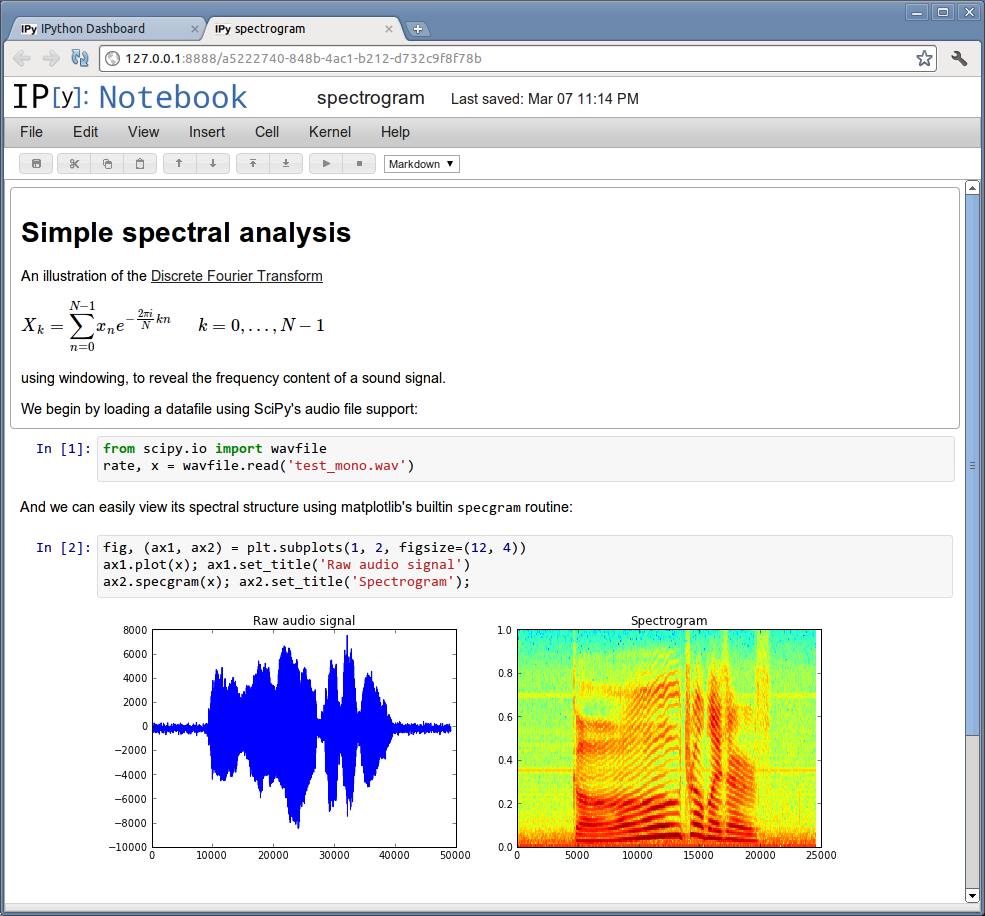
\includegraphics[width=3.2in]{fig/ipython-notebook-specgram.png}\par
  \end{centering}

  \caption{\label{fig:IPython-notebook}The web-based IPython Notebook combines
    explanatory text, mathematics, multimedia, code and the results from
    executing the code.}
\end{figure}

The driving idea behind the IPython Notebook is to enable researchers to move
fluidly between all the phases of the research life cycle described in
§~\ref{subsec:lifecycle}.  If the environment where we conduct our
exploratory research can also support all subsequent stages of this cycle, and
does so while smoothly integrating with the version control and process
practices we've previously espoused, the likelihood that a final published
result will be reproducible increases significantly.  The Notebook system is
designed around two central ideas: (a) an openly specified protocol to control
an interactive computational engine, and (b) an equally open format to record
these interactions between the user and the computational engine, including the
results produced by the computations.

Before diving into the specifics of these two ideas, we note that the above
design is independent of the Python language: while IPython started its life as
a Python-specific project, the vision of the Notebook system is
language-agnostic.  First, while working in IPython, users can mark entire code
blocks for execution via a separate language by using a special syntax on the
block's first line: a user can for example start a block \texttt{\%\%R},
\texttt{\%\%octave}, \texttt{\%\%bash} or \texttt{\%\%ruby} and IPython will
execute the entire block with the respective system.  The development community
is also busy implementing similar support for new and experimental
scientific languages such as Julia, enabling a user to control from a single
IPython notebook a workflow that combines the most commonly used high-level
languages in modern scientific computing.  Second, an \emph{entire notebook}
can be executed in a different language if a remote engine (referred to as a
\emph{kernel}) exists that implements the interaction protocol.  As of this
writing, prototype kernels are being developed for Ruby, JavaScript, R, and
Julia.

The IPython architecture provides a way to capture, version control, re-execute,
and convert into other output formats, any computational session.  Notebooks
can be shared with colleagues in their native form for re-execution or
converted into HTML, \LaTeX{}, or PDF formats for reading and dissemination.  They
can be used in slideshow mode to give presentations that remain connected to a
live computation and can be exported into plain scripts for traditional
execution outside of the IPython framework.

The IPython protocol consists of messages in JSON (JavaScript Object Notation)
format that encode all actions that an interactive user can request of a
computational kernel, such as executing code, transferring data, or sending
results, among many others.  While this protocol is implemented in IPython, it
can be independently implemented to provide new kernels also able to interact
with the notebook interface and clients.  The notebook file format is a simple
JSON data structure that contains a list of cells.  A cell can contain either
text or code, and code cells can also have the output corresponding to the
execution.  All sub-structures in the notebook format (the entire notebook as
well as the individual cells) have attached flexible metadata containers; this
metadata can be used by post-processing tools.  The file format stores the
communication protocol's payloads unmodified, so it can be thought of as a
structured and filtered log (since the user chooses what to keep while working
interactively) of the computation.  

The IPython project has taken elements pioneered by the Mathematica and Sage
notebooks and created a generic protocol and file format to control and record
literate computing sessions in any programming language.  This was a deliberate
choice in contrast to the literate programming approach: by providing a tool
that operates close to the live workflow of research computing (in contrast to
the batch-processing mode encouraged by classic literate programming tools),
the resulting documents are immediately reproducible sessions that can be
published in their own right or as companion materials to a traditional
manuscript.  Given how IPython also includes support for parallel computing,
which we don't discuss here in the interest of conciseness, the system provides
an end-to-end environment for the creation of reproducible research.

The real-world possibilities this offers were demonstrated during a
collaboration in 2012 between the IPython team, a microbiology team led by Rob
Knight from the University of Colorado and Greg Caporaso from the University of
Northern Arizona, and Justin Riley from MIT who created the
StarCluster\footnote{\url{http://star.mit.edu/cluster}} system for deployment
and control of parallel resources on Amazon's EC2 cloud platform.  As part of
an NIH-funded workshop to explore the future of genomics data analysis in the
cloud, this combined team collaborated on creating a fully parallelized
analysis comparing the predictive behavior of different sizes and locations of
gene sequence reads when reconstructing phylogenetic trees.  The
microbiologists had developed a serial prototype of this idea using their Qiime
libraries \cite{caporaso2010qiime}, but a large-scale analysis with a full
dataset would require roughly a month of CPU time on a single workstation.  By
locating the IPython Notebook server on Amazon cloud instances, the entire team
was able to log into a single instance and by editing the code directly in the
cloud, in a single day turn this prototype into a set of production notebooks
that would execute the analysis in parallel using multiple Amazon servers.
Once the parallel code was tested, it became evident that there was not only an
interesting example of using cloud technologies for rapid development of
research ideas but also a biologically relevant finding; within a week the team
had completed a more extensive run using 24 hours of execution on 32 nodes and
submitted a manuscript for publication \cite{RWM+12}.  This paper is now
accompanied by all of the IPython notebooks that enable any reader to fully
reproduce our analysis, change parameters and question our assumptions, without
having to re-implement anything or be hampered by lack of access to the code
and data.  We have made available not only the final notebooks, but also the
Amazon Virtual Machine Images (data files that represent a virtual computer on
Amazon's cloud platform), so that the entire analysis can literally be
re-executed under identical conditions by anyone with an Amazon account.

This example, anecdotal as it may be, indicates the validity of the vision
we propose here: that by providing tools that encompass the entire cycle of
research, from exploration to large-scale parallel production and publication,
we can provide the scientific community with results that are immediately
accessible to others and reproducible, seeding the continued evolution of the
research process.

The IPython project has also developed tools to make it easy to share and
disseminate content created as notebooks in a variety of forms.  The Notebook
Viewer\footnote{\url{http://nbviewer.org}} is an online service that renders
\emph{any} publicly available IPython notebook as a web page.  This enables
users to share notebooks by simply putting them online and pointing colleagues
to the rendered webpage.  The same technology that powers the notebook viewer
service can also generate HTML files suitable for inclusion in other websites,
in particular, blogs.  Since a lot of rapid technical communication is
happening today on the Internet via blogs, this is an important aspect of
linking reproducible research to the rapid feedback cycle of web-based
discussion.  With a single command, a user can convert a notebook file into
HTML ready for posting to a blog, and this is already being used by scientists
to write both short technical posts and also more complex materials: Jose
Unpingco, a researcher with the US Department of Defense, is currently working
on a book titled \emph{Python for Signal Processing}, and this book is
available during writing as a GitHub
repository.\footnote{\url{http://github.com/unpingco/Python-for-Signal-Processing}}
This repository contains a series of IPython notebooks so that readers can
directly execute the code in the book, and they are also being published as a
series of blog posts as they become
available,\footnote{\url{http://python-for-signal-processing.blogspot.com}} so
readers can comment and discuss with the author throughout the process of book
development, and they can do so based directly on the actual code that creates
all the examples in the book.

The signal processing book is, to our knowledge, the first example of a full
book being written as a collection of executable IPython notebooks, but this
follows a tradition created by Mathematica, whose documentation is itself a
collection of executable Notebooks.  Furthermore, in recent years Rob Beezer,
from the University of Puget Sound, has developed a popular Introductory Linear
Algebra book \cite{beezer2009first} that is based on the Sage system and also
combines the mathematics and text with code that can be directly executed and
modified by the readers.  This ability to ``close the loop'' between what the
authors had on their screens and what their readers can execute themselves is
an important element of the movement towards reproducibility in research.

As a concrete implementation of the ideas of reproducible research using the
tools we've described in this chapter, during the ongoing process of research
itself, we can point to work being carried by a collaboration where one of us
(FP) is a member, on novel ways to model the mathematical structure of the
signal generated by MRI devices in the imaging of water diffusion in the
brain.  This work, as yet unpublished, is being developed as an open repository
on GitHub\footnote{\url{http://github.com/fperez/spheredwi}} where all code
for our research is posted during writing, all computational experiments are
created as IPython notebooks, and submitted manuscripts are created directly
from the code and notebooks (along with additional narrative written by hand).

The above tools are also playing a central role in the last stage of the
computational research life cycle, education.  We will increase our chance that
the next generation of scientists adopts improved reproducibility practices if
we educate them with the same tools that we use for everyday research, and a
couple of modern efforts that aim to bring improved computational literacy to
scientific research have adopted the IPython notebook.  Software
Carpentry\footnote{\url{http://software-carpentry.org}} is a project funded by
the Alfred P. Sloan Foundation and led by Greg Wilson at the Mozilla Foundation
whose motto is Richard Feynman's famous ``What I cannot create, I do not
understand.''  They produce, with rigorous follow-up and assessment, workshops
aimed at working scientists (typically graduate students and postdoctoral
researchers, but always open to broad audiences) and whose purpose is to
instill in them a collection of skills and best practices for effectively using
computing as a daily research tool.  The Software Carpentry workshops cover
topics ranging from the basics of the Unix shell to version control, Makefile
automation of processes and basics of scientific Python including data analysis
and visualization.  They have recently adopted the IPython Notebook as the base
system for teaching the scientific Python parts of their curricula, and provide
the IPython team with direct feedback on its strengths and weaknesses as an
educational tool.  In a similar vein, Josh Bloom from the astronomy department
at UC Berkeley has led, for a number of years, 3-day workshops on the use of
Python as a tool for scientific
computing.\footnote{\url{http://pythonbootcamp.info}}  These are open to the
entire campus community and followed by an optional for-credit seminar where
students learn more advanced skills for using Python as a research tool.  F.
Pérez and other members of the IPython team at UC Berkeley regularly lecture in
the bootcamps and courses, where the notebook is the means for delivery of
course materials and interactive lecturing.  While we have identified a number
of weaknesses and areas for improvement, we have also found this environment to
be markedly superior to all previous tools we had used in the past for teaching
in similar contexts.

As these capabilities in IPython reach wider usage, with scientists now
developing complete books and lecture series based on the system, we are
considering a number of new challenges and questions introduced by these
capabilities.  The interactive computing model is a fluid and natural one, but
we need to find ways to extend it into the development of longer-term
production codes that are robust, documented, tested and integrated into
reusable libraries.  This means bridging the gap between a \emph{scripting}
mentality and a \emph{developer} one, and while we have already made progress on
that front in IPython, many questions remain open for the future.

\section{Conclusion}\label{conclusion}

As research grows increasingly dependent on computing, it becomes critical for
our computational resources to be developed with the same rigor, review,
and access, as the results they support. In particular, we believe that
reproducibility in computational research requires: (1) sharing of scientific
software, data, and knowledge necessary for reproducible research; (2)
readable, tested, validated, and documented software as the basis for reliable
scientific outcomes; (3) high standards of computational literacy in the
education of mathematicians, scientists, and engineers; and (4) open source
software developed by collaborative, meritocratic communities of practice.

Achieving these goals will not be easy.  It requires changing the educational
process for new scientists, the incentive models for promotions and rewards,
the publication system \cite{neylon2012changing}, and more. In this chapter, we
focused on the need for an open source ecosystem for scientific computing
developed by communities of practice.  We then introduced several tools and
practices necessary---but not sufficient---for reliable code that can be the
basis of reproducible research.  We illustrated these ideas with examples of
how they have been applied and advanced in the open source scientific Python
community.  Finally, we presented the IPython project's combination of
interactivity, distributed and remote computing features, and literate
computing functionality as a natural integration point for the computational
research life cycle in order to make it more fluid, efficient, and
reproducible.

We emphasize that the mechanical reproduction of computational results
is not an end in itself.  The ultimate goal is to bring the rigor, openness,
culture of validation and collaboration, as well as other aspects of
reproducible research to our everyday computational practices. This is not a
goal we will happily attain one day and then move on to pursue another;
it must become and remain an ongoing part of our scientific practice.

\section*{Acknowledgments}

We would like to thank all the members of the scientific Python community as
well as the many scientists from various labs whose work and ideas have inspired
what we have presented here.  John D. Hunter, to whom this chapter is dedicated,
created the matplotlib graphics library that has been a central pillar of the
Scientific Python ecosystem; his tragic early passing in 2012 was a personal
blow to the authors as well as a loss to our community.  Brian Granger and Min
Ragan-Kelley have worked closely with FP on the development of IPython for a
number of years and are responsible for many of the ideas that the project
embodies.  Matthew Brett has through long collaboration and patient
discussion helped clarify and refine many of the ideas presented in this
chapter.  Titus Brown, Vincent Carey, Paul Ivanov, Jean-Baptiste Poline, and
Stéfan van der Walt provided valuable feedback on drafts of this chapter.

\bibliographystyle{plain}
\bibliography{millman-perez}

\end{document}
